\uuid{PMwZ}
\exo7id{5714}
\titre{exo7 5714}
\auteur{rouget}
\organisation{exo7}
\datecreate{2010-10-16}
\isIndication{false}
\isCorrection{true}
\chapitre{Calcul d'intégrales}
\sousChapitre{Intégrale impropre}
\module{Analyse}
\niveau{L1}
\difficulte{}

\contenu{
\texte{
Etudier l'existence des intégrales suivantes.

\begin{center}
\begin{tabular}{ll}
\textbf{1) (***) I} $\int_{2}^{+\infty}\frac{1}{x^a\ln^bx}\;dx$ (Intégrales de \textsc{Bertrand})&\textbf{2) (**)} $\int_{0}^{\pi/2}(\tan x)^a\;dx$\\
\rule[-6mm]{0mm}{14mm}\textbf{3) (**)} $\int_{1}^{+\infty}\left(\left(1+\frac{1}{x}\right)^{1+\frac{1}{x}}- a-\frac{b}{x}\right) dx$& 
\textbf{4) (***)} $\int_{0}^{+\infty}\frac{1}{x^a(1+x^b)}\;dx$
\end{tabular}
\end{center}
}
\reponse{
Pour tout couple de réels $(a,b)$, la fonction $f~:~x\mapsto\frac{1}{x^a\ln^bx}$ est continue et positive sur $[2,+\infty[$. Etudions l'intégrabilité de $f$ au voisinage de $+\infty$.

\textbf{1er cas.} Si $a > 1$,  $x^{(a+1)/2}f(x)=\frac{1}{x^{(a-1)/2}\ln^bx}\underset{x\rightarrow+\infty}{\rightarrow}0$ car  $\frac{a-1}{2}>0$ et d'après un théorème de croissances comparées. Donc $f(x)\underset{x\rightarrow+\infty}{=}o\left(\frac{1}{x^{(a+1)/2}}\right)$. Comme $\frac{a+1}{2}>1$, la fonction $x\mapsto\frac{1}{x^{(a+1)/2}}$ est intégrable sur un voisinage de $+\infty$ et il en est de même de $f$. Dans ce cas, $f$ est intégrable sur $[2,+\infty[$.

\textbf{2ème cas.} Si $a <1$,  $x^{(a+1)/2}f(x)=\frac{x^{(1-a)/2}}{\ln^bx}\underset{x\rightarrow+\infty}{\rightarrow}+\infty$ car  $\frac{1-a}{2}>0$ et d'après un théorème de croissances comparées. Donc $f(x)$ est prépondérant devant $\frac{1}{x^{(a+1)/2}}$ en $+\infty$. Comme $\frac{a+1}{2}<1$, la fonction $x\mapsto\frac{1}{x^{(a+1)/2}}$ n'est pas intégrable sur un voisinage de $+\infty$ et il en est de même de $f$. Dans ce cas, $f$ n'est pas intégrable sur $[2,+\infty[$.

\textbf{3ème cas.} Si $a = 1$. Pour $X > 2$ fixé , en posant $t =\ln x$ et donc $dt=\frac{dx}{x}$ on obtient

\begin{center}
$\int_{2}^{X}\frac{1}{x\ln^b}\;dx=\int_{\ln2}^{\ln X}\frac{dt}{t^b}$.
\end{center}

Puisque $\ln X$ tend vers $+\infty$ quand $X$ tend vers $+\infty$ et que les fonctions considérées sont positives, f est intégrable sur $[2, +\infty[$ si et seulement si $b > 1$.

En résumé , 

\begin{center}
\shadowbox{
la fonction $x\mapsto\frac{1}{x^a\ln^bx}$ est intégrable sur $[2,+\infty[$ si et seulement si $a > 1$ ou ($a=1$ et $b > 1$).
}
\end{center}

(En particulier, la fonction $x\mapsto\frac{1}{x\ln x}$ n'est pas intégrable sur voisinage de $+\infty$ bien que négligeable devant $\frac{1}{x}$ en $+\infty$).
Pour tout réel $a$,  la fonction $f~:~x\mapsto(\tan x)^a$ est continue et strictement positive sur $\left]0,\frac{\pi}{2}\right[$. De plus, pour tout réel $x$ de$\left]0,\frac{\pi}{2}\right[$, on a $f\left(\frac{\pi}{2}-x\right) =\frac{1}{f(x)}$.

\textbullet~\textbf{Etude en $0$ à droite.} $f(x)\underset{x\rightarrow0}{\sim}x^a$. Donc $f$ est intégrable sur un voisinage de $0$ à droite si et seulement si $a > -1$.

\textbullet~\textbf{Etude en $\frac{\pi}{2}$ à gauche.}$f(x)=\frac{1}{f\left(\frac{\pi}{2}-x\right)}\underset{x\rightarrow\frac{\pi}{2}}{\sim}\left(\frac{\pi}{2}-x\right)^{-a}$. Donc $f$ est intégrable sur un voisinage de $\frac{\pi}{2}$ à gauche si et seulement si $a < 1$. 

En résumé, $f$ est intégrable sur $\left]0,\frac{\pi}{2}\right[$ si et seulement si $-1 < a < 1$.
Pour $x\geqslant1$, $1+\frac{1}{x}$ est défini et strictement positif. Donc pour tout couple $(a,b)$ de réels, la fonction $f~:~ x\mapsto\left(1+\frac{1}{x}\right)^{1+\frac{1}{x}}-a -\frac{b}{x}$  est continue sur $[1,+\infty[$.

En $+\infty$, $\left(1+\frac{1}{x}\right)\ln\left(1+\frac{1}{x}\right) =\left(1+\frac{1}{x}\right)\left(\frac{1}{x}+O\left(\frac{1}{x^2}\right)\right)=\frac{1}{x}+O\left(\frac{1}{x^2}\right)$. Donc 

\begin{center}
$f(x)\underset{x\rightarrow+\infty}{=}(1-a)+\frac{1-b}{x}+O\left(\frac{1}{x^2}\right)$.
\end{center}

\textbullet~Si $a\neq 1$, $f$ a une limite réelle non nulle en $+\infty$ et n'est donc pas intégrable sur $[1,+\infty[$.

\textbullet~Si $a = 1$ et $b\neq 1$, $f(x)\underset{x\rightarrow+\infty}{\sim}\frac{1-b}{x}$. En particulier, $f$ est de signe constant sur un voisinage de $+\infty$ et n'est pas intégrable sur $[1,+\infty[$.

\textbullet~Si $a = b = 1$, $f(x)\underset{x\rightarrow+\infty}{=}O\left(\frac{1}{x^2}\right)$ et dans ce cas, $f$ est intégrable sur $[1,+\infty[$.

En résumé, $f$ est intégrable sur $[1,+\infty[$ si et seulement si $a = b = 1$.
Pour tout couple $(a,b)$ de réels, la fonction $f~:~ x\mapsto\frac{1}{x^a(1+x^b)}$ est continue et positive sur $]0,+\infty[$.

\textbullet~\textbf{Etude en $0$.} 

-Si $b>0$, $f(x)\underset{x\rightarrow0}{\sim}\frac{1}{x^a}$, et donc $f$ est intégrable sur un voisinage de $0$ si et seulement si $a<1$,

-si $b=0$, $f(x)\underset{x\rightarrow0}{\sim}\frac{1}{2x^a}$, et donc $f$ est intégrable sur un voisinage de $0$ si et seulement si $a<1$,

-si $b<0$, $f(x)\underset{x\rightarrow0}{\sim}\frac{1}{x^{a+b}}$, et donc $f$ est intégrable sur un voisinage de $0$ si et seulement si $a+b<1$.

\textbullet~\textbf{Etude en $+\infty$.} 

-Si $b>0$, $f(x)\underset{x\rightarrow0}{\sim}\frac{1}{x^{a+b}}$, et donc $f$ est intégrable sur un voisinage de $+\infty$ si et seulement si $a+b>1$,

-si $b=0$, $f(x)\underset{x\rightarrow0}{\sim}\frac{1}{2x^a}$, et donc $f$ est intégrable sur un voisinage de $+\infty$ si et seulement si $a>1$,

-si $b<0$, $f(x)\underset{x\rightarrow0}{\sim}\frac{1}{x^{a}}$, et donc $f$ est intégrable sur un voisinage de $+\infty$ si et seulement si $a>1$.

En résumé, $f$ est intégrable sur $]0,+\infty[$ si et seulement si (($b\geqslant0$ et $a<1$) ou ($b<0$ et $a+b<1$)) et (($b>0$ et $a+b>1$) ou ($b\leqslant0$ et $a>1$)) ce qui équivaut à ($b>0$ et $a+b>1$ et $a<1$) ou ($b<0$ et $a>1$ et $a+b<1$).

Représentons graphiquement l'ensemble des solutions. La zone solution est la zone colorée.

$$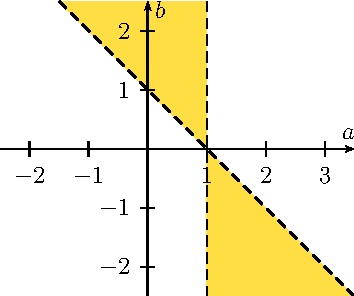
\includegraphics{../images/pdf/PMwZ-1.pdf}$$
}
}
